
% $Header: /cvsroot/latex-beamer/latex-beamer/solutions/conference-talks/conference-ornate-20min.en.tex,v 1.6 2004/10/07 20:53:08 tantau Exp $
\PassOptionsToPackage{pdfpagelabels=false}{hyperref}
\documentclass
%[handout] % Enable this opption if you want a compact printout of the talk for distribution.
{beamer}

% This file is a solution template for:

% - Talk at a conference/colloquium.
% - Talk length is about 20min.
% - Style is ornate.



% Copyright 2004 by Till Tantau <tantau@users.sourceforge.net>.
%
% In principle, this file can be redistributed and/or modified under
% the terms of the GNU Public License, version 2.
%
% However, this file is supposed to be a template to be modified
% for your own needs. For this reason, if you use this file as a
% template and not specifically distribute it as part of a another
% package/program, I grant the extra permission to freely copy and
% modify this file as you see fit and even to delete this copyright
% notice. 


\mode<presentation>
{
  \usetheme{Warsaw}
	\usecolortheme[RGB={0,102,51}]{structure}
  % or ...

  %\setbeamercovered{transparent}
  % or whatever (possibly just delete it)
}


\usepackage[english]{babel}
% or whatever

\usepackage[latin1]{inputenc}
% or whatever

\usepackage{times}
\usepackage[T1]{fontenc}
\usepackage{pgf,tikz}
\usepackage{color}
\usepackage{xcolor}
\usepackage{cases}

\def\mathunderline#1#2{\color{#1}\underline{{\color{black}#2}}\color{black}}
\usetikzlibrary{arrows}
\usetikzlibrary{calc}
\newcommand\scalemath[2]{\scalebox{#1}{\mbox{\ensuremath{\displaystyle #2}}}}
\newcommand{\R}{{\mathbb R}}
\newcommand{\Q}{{\mathbb Q}}
\newcommand{\C}{{\mathbb C}}
\newcommand{\N}{{\mathbb N}}
\newcommand{\Z}{{\mathbb Z}}
\newcommand{\Fr}{{\text{Fr}}}
\newcommand{\LCM}{\text{LCM}}
\newcommand{\multideg}{\text{multideg}}
\newcommand{\ord}{\text{ord}}
\newcommand{\Irr}{\text{Irr}}
% Or whatever. Note that the encoding and the font should match. If T1
% does not look nice, try deleting the line with the fontenc.

\definecolor{ffffff}{rgb}{1.0,1.0,1.0}
\definecolor{wwwwqq}{rgb}{0.4,0.4,0}
\definecolor{zzqqtt}{rgb}{0.6,0,0.2}
\definecolor{zzttqq}{rgb}{0.6,0.2,0}
\definecolor{qqwwcc}{rgb}{0,0.4,0.8}
\definecolor{fffftt}{rgb}{1,1,0.2}
\definecolor{qqqqff}{rgb}{0,0,1}
\definecolor{qqzzqq}{rgb}{0,0.6,0}
\definecolor{ffqqqq}{rgb}{1,0,0}
\definecolor{uququq}{rgb}{0.25,0.25,0.25}

\title[Dushnik-Miller Embeddings and some Limitations] % (optional, use only with long paper titles)
{An Introduction to Poset Dimensions}


\author[McGuire] % (optional, use only with lots of authors)
{Trevor McGuire}
% - Give the names in the same order as the appear in the paper.
% - Use the \inst{?} command only if the authors have different
%   affiliation.

\institute[NDSU] % (optional, but mostly needed)
{
  %
  Department of Mathematics\\
  North Dakota State University\\
  Fargo, ND}
  
% - Use the \inst command only if there are several affiliations.
% - Keep it simple, no one is interested in your street address.

\date[AMS2007] % (optional, should be abbreviation of conference name)
{Combinatorics Seminar, NDSU, September 2015}
% - Either use conference name or its abbreviation.
% - Not really informative to the audience, more for people (including
%   yourself) who are reading the slides online

 



% If you have a file called "university-logo-filename.xxx", where xxx
% is a graphic format that can be processed by latex or pdflatex,
% resp., then you can add a logo as follows:

% \pgfdeclareimage[height=0.5cm]{university-logo}{university-logo-filename}
% \logo{\pgfuseimage{university-logo}}



% Delete this, if you do not want the table of contents to pop up at
% the beginning of each subsection:



% If you wish to uncover everything in a step-wise fashion, uncomment
% the following command: 

%\beamerdefaultoverlayspecification{<+->}


\begin{document}

\begin{frame}
  \titlepage
\end{frame}

%\begin{frame}
  %\frametitle{Outline}
%  \tableofcontents
  % You might wish to add the option [pausesections]
%\end{frame}


% Structuring a talk is a difficult task and the following structure
% may not be suitable. Here are some rules that apply for this
% solution: 

% - Exactly two or three sections (other than the summary).
% - At *most* three subsections per section.
% - Talk about 30s to 2min per frame. So there should be between about
%   15 and 30 frames, all told.

% - A conference audience is likely to know very little of what you
%   are going to talk about. So *simplify*!
% - In a 20min talk, getting the main ideas across is hard
%   enough. Leave out details, even if it means being less precise than
%   you think necessary.
% - If you omit details that are vital to the proof/implementation,
%   just say so once. Everybody will be happy with that.

\section{Dushnik-Miller Dimension}



%\subsection{Background}

\begin{frame}
  \frametitle{Posets}
 
 For the sake of formality, we will define a poset.

\pause
\begin{definition} 
456
\end{definition}

\end{frame}

\begin{frame}

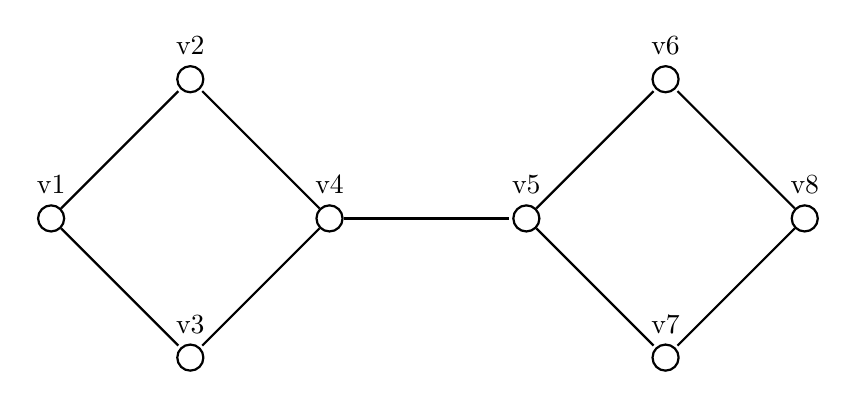
\begin{tikzpicture}[>=stealth',shorten >=1pt,auto,node distance=2.5cm,
                    thick,main node/.style={circle,draw,font=\sffamily\Large\bfseries}]
\node[main node] (1) [label={v1}] {};
\node[main node] (2) [above right of=1, label={v2}] {};
\node[main node] (3) [below right of=1, label={v3}] {};
\node[main node] (4) [above right of=3, label={v4}] {};
\node[main node] (5) [right of =4, label={v5}] {};
\node[main node] (6) [above right of =5, label={v6}] {};
\node[main node] (7) [below right of =5, label={v7}] {};
\node[main node] (8) [above right of =7, label={v8}] {};

\path[thick]
  (1) edge (2)
      edge (3)
  (4) edge (2)
      edge (3)
      edge (5)
  (5) edge (6)
      edge (7)
  (8) edge (6)
      edge (7);

      
\end{tikzpicture}


\end{frame}

\begin{frame}
\begin{center}
\LARGE Thank You!
\end{center}
\end{frame}
\end{document}


